\section{Detailed SSC Results}
\label{app:ssc_detailed_results}

Additional class-wise and altitude-wise SSC results are provided here to keep the main paper focused on the principal trends.

\begin{figure}[!htbp]
\centering
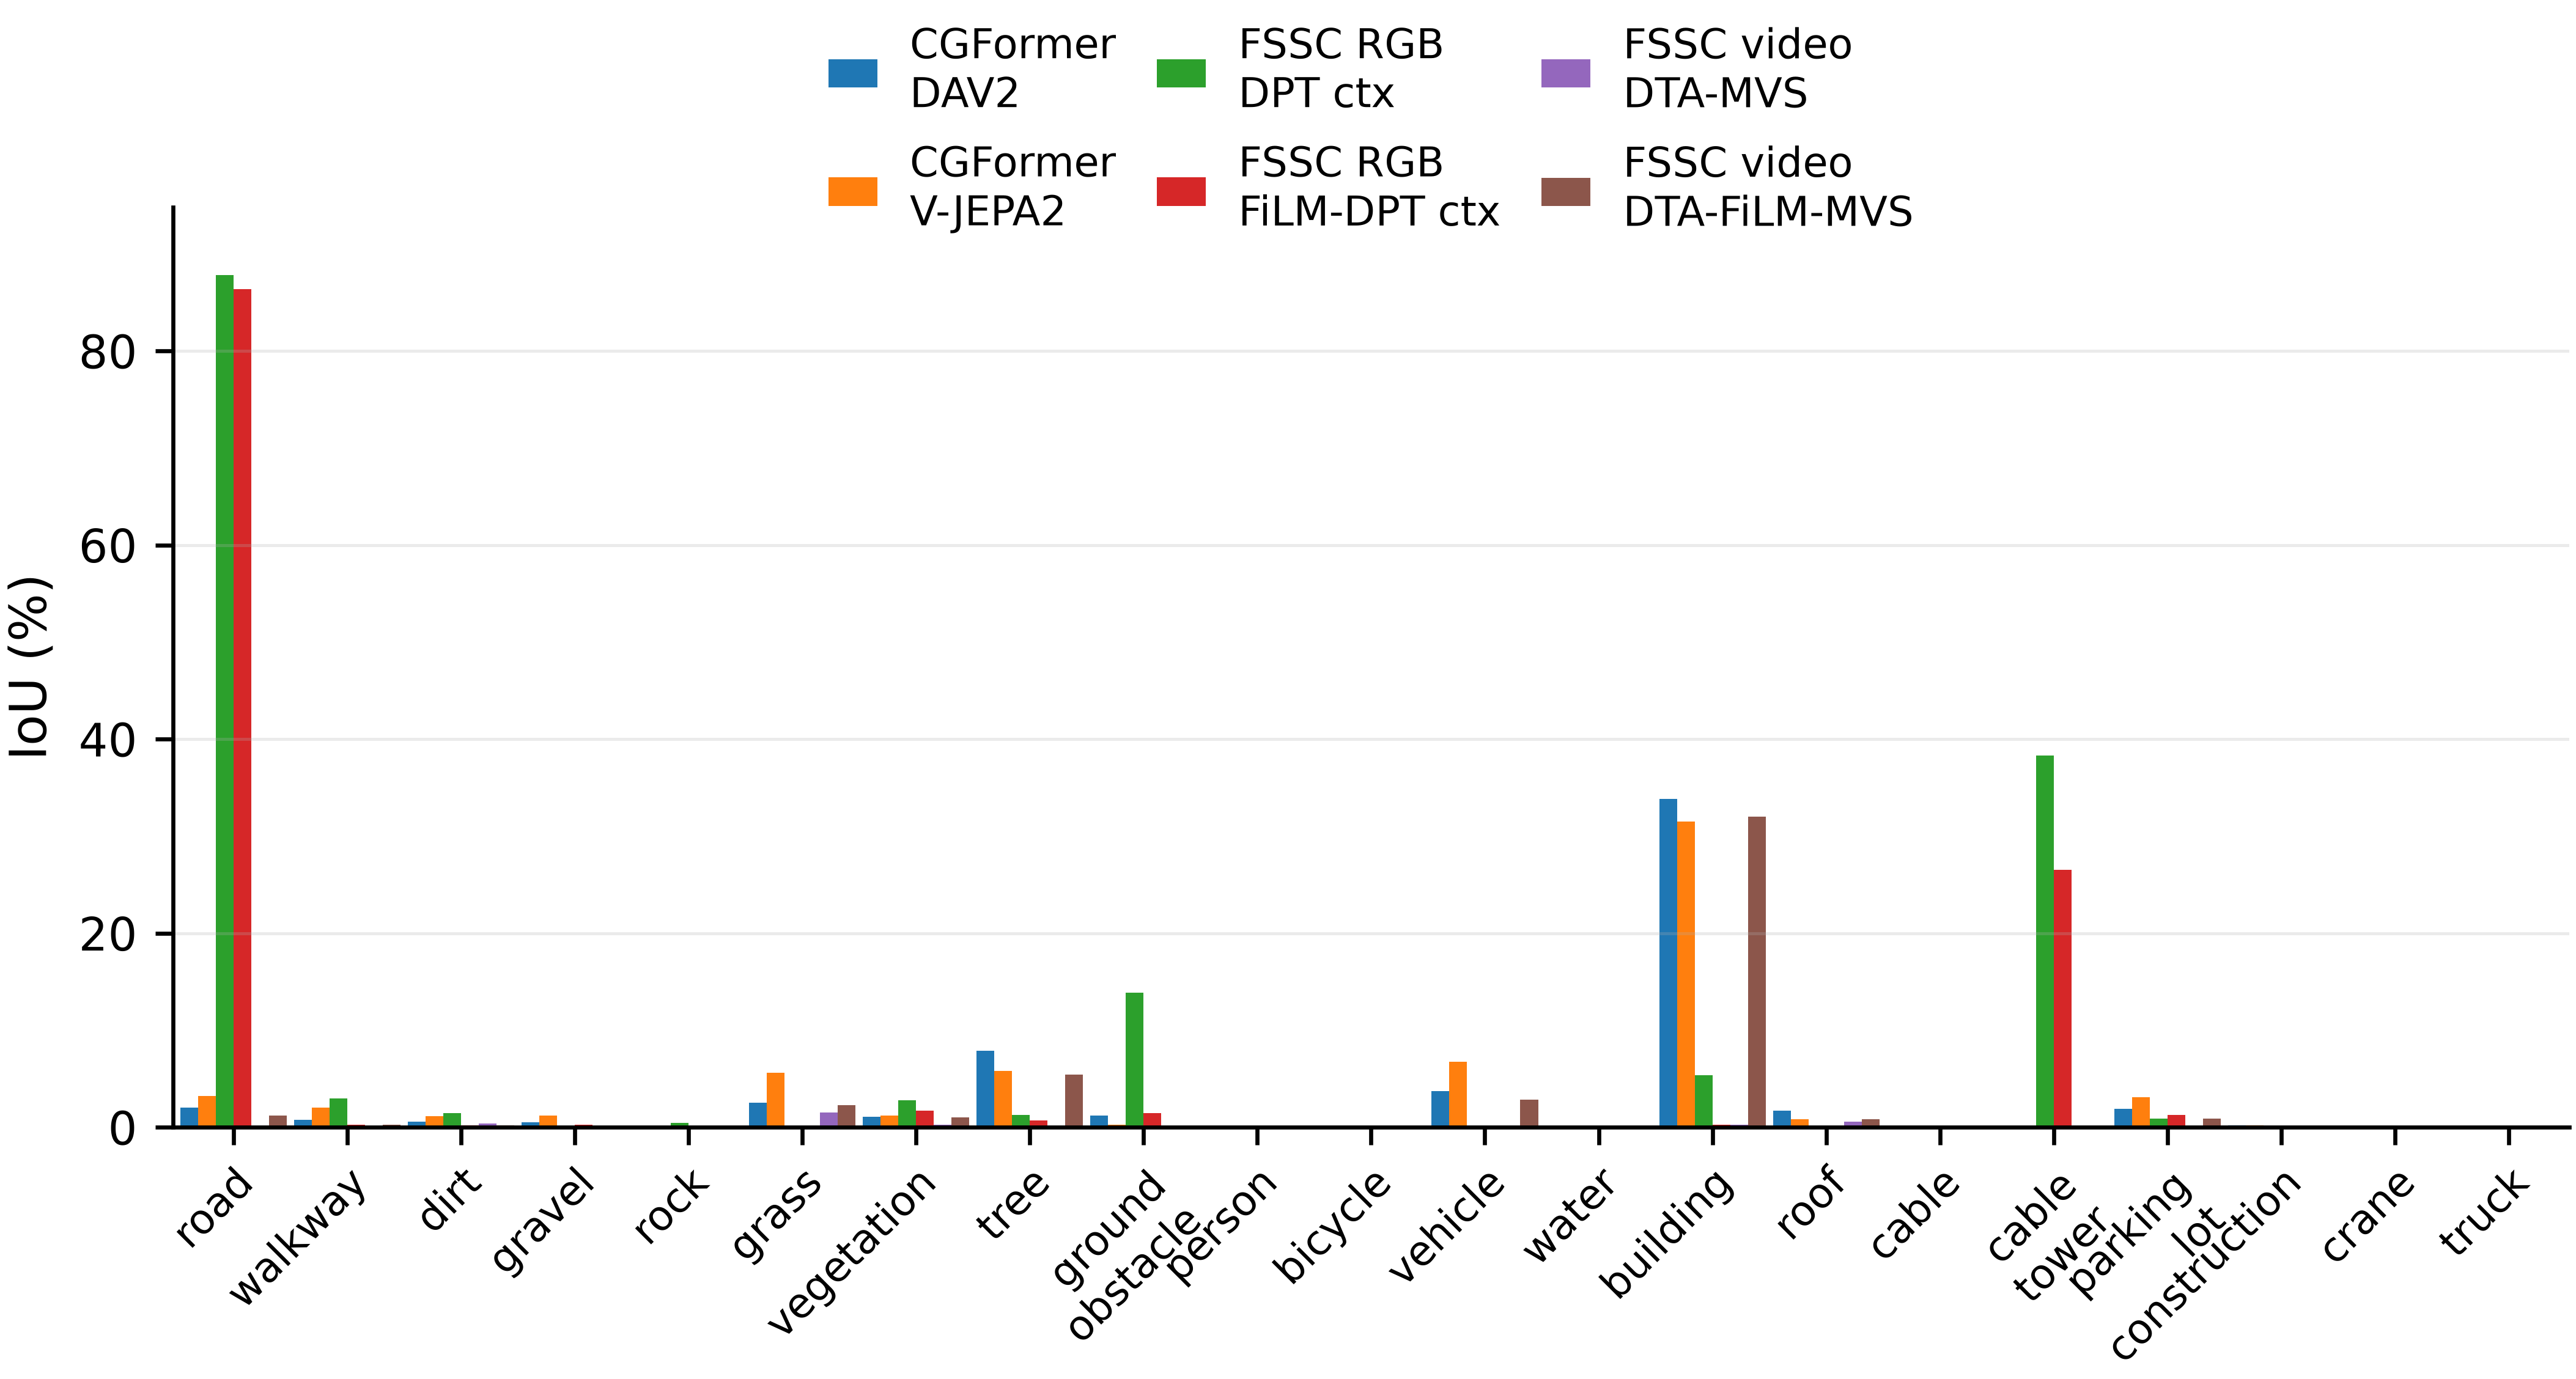
\includegraphics[width=0.96\linewidth]{content/images/ssc/occufly_ssc_per_class_iou_bar_chart.png}
\caption{OccuFly SSC per-class IoU bar chart for the evaluated CGFormer and FoundationSSC variants.}
\label{fig:occufly_ssc_per_class_iou_bar_chart}
\end{figure}

\begin{figure}[!htbp]
\centering
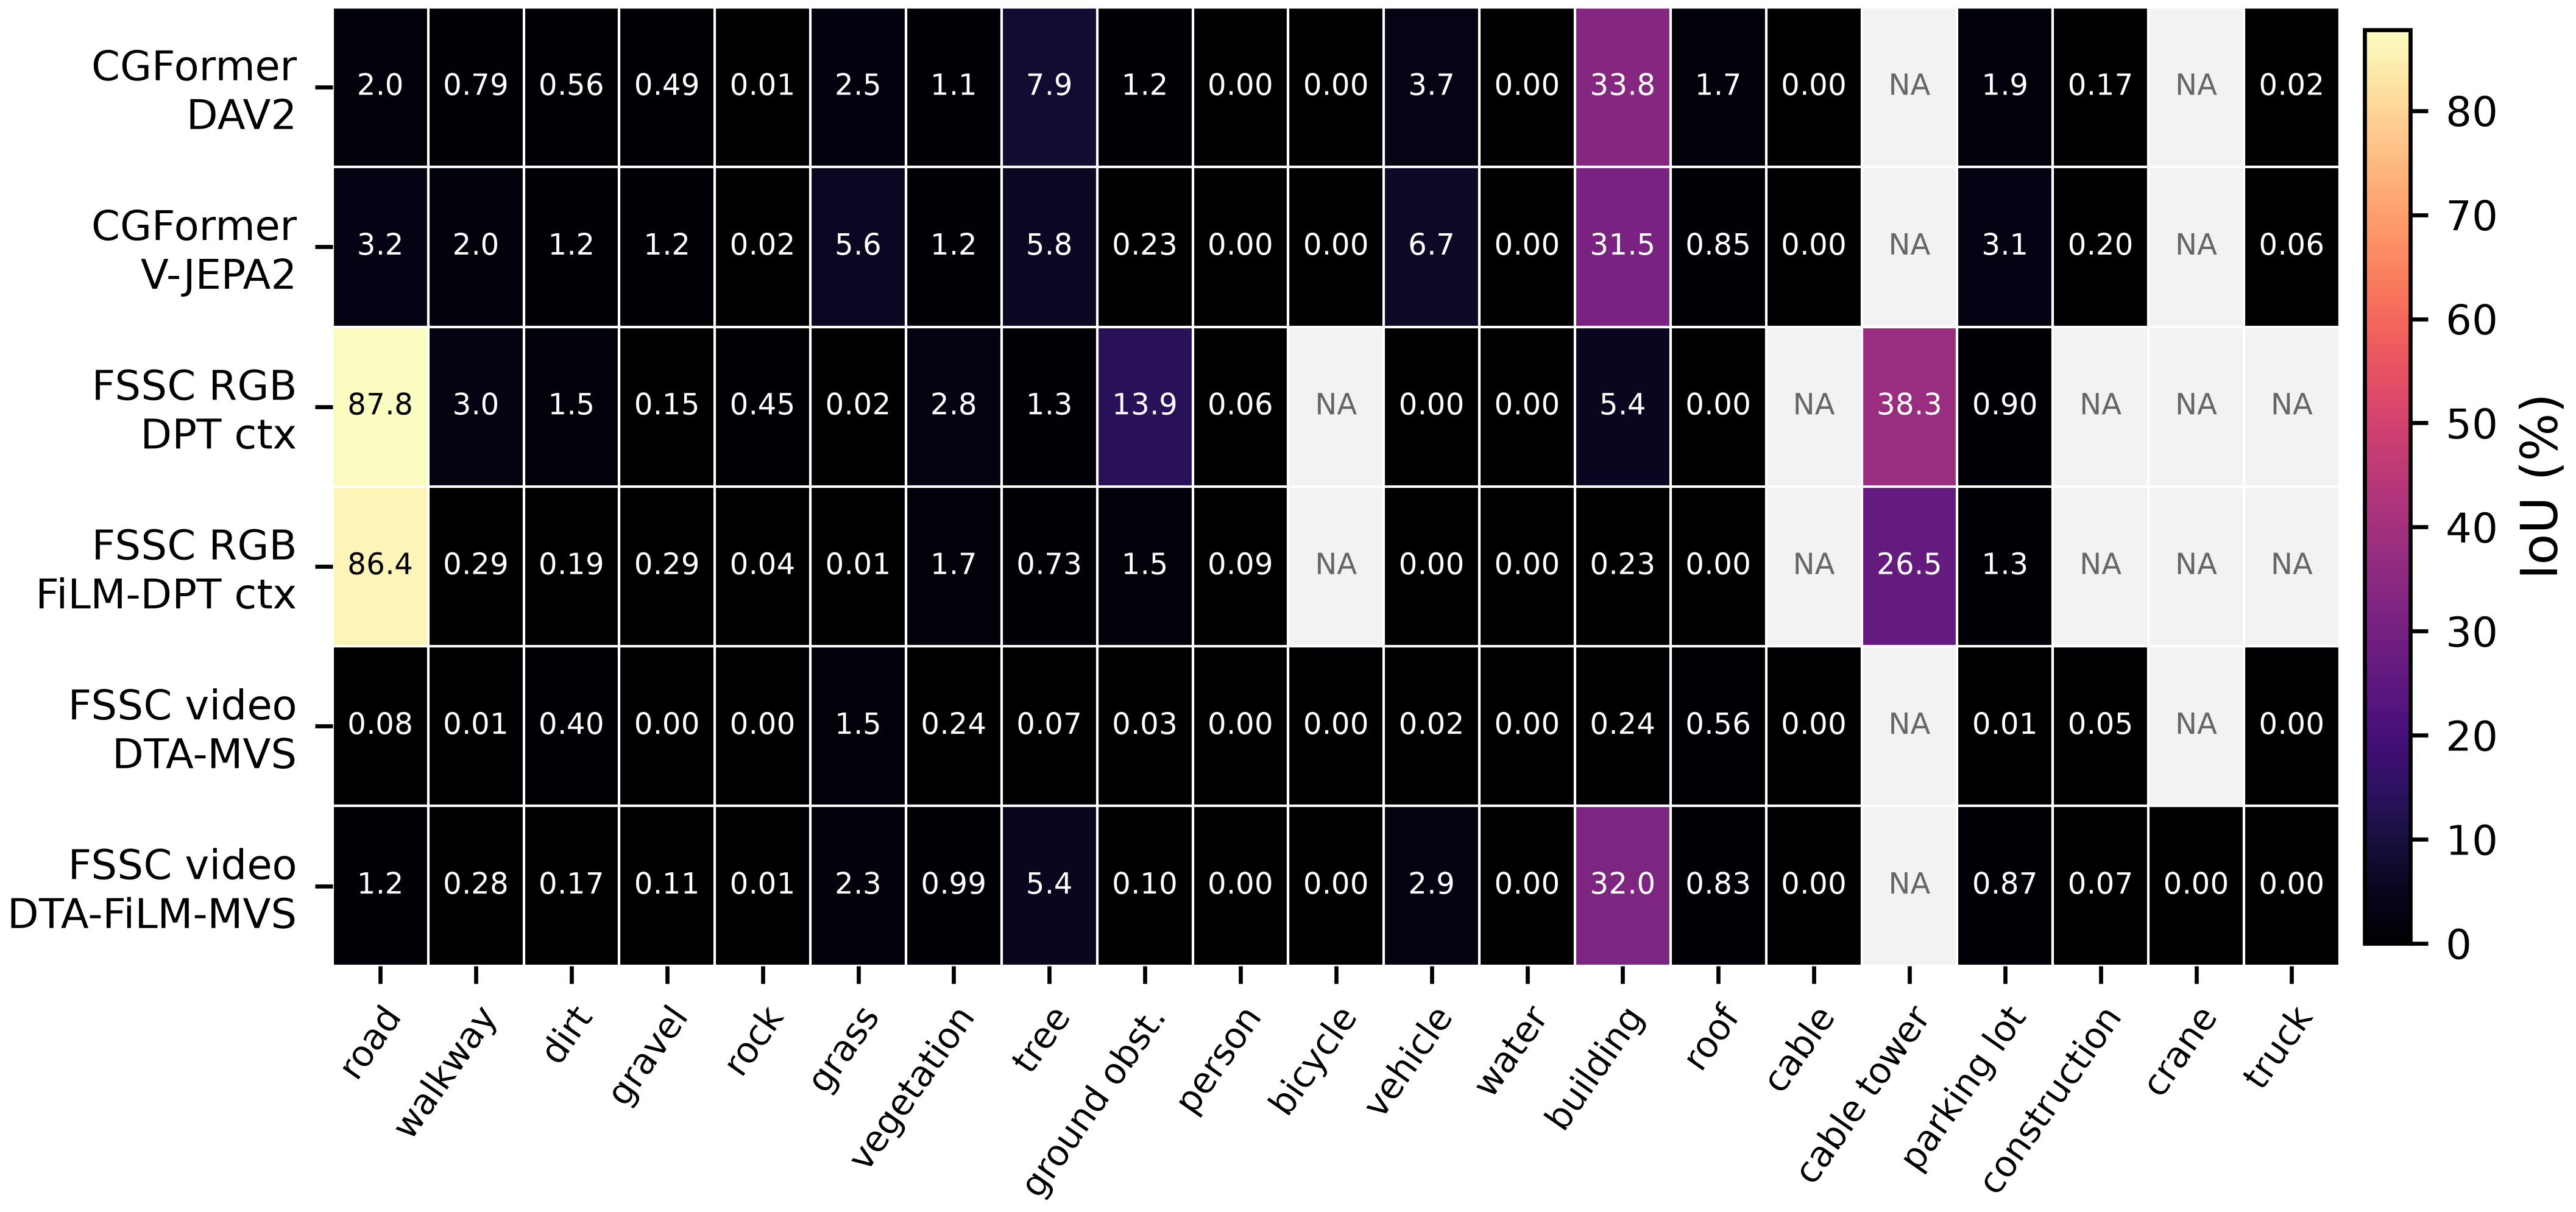
\includegraphics[width=0.96\linewidth]{content/images/ssc/occufly_ssc_per_class_iou_heatmap.png}
\caption{OccuFly SSC per-class IoU heatmap for the evaluated CGFormer and FoundationSSC variants.}
\label{fig:occufly_ssc_per_class_iou_heatmap}
\end{figure}

\begin{table}[!htbp]
\centering
\caption{OccuFly SSC benchmark comparison by altitude. Published Symphonies and DISC values follow OccuFly Table~4~\cite{gross2026occufly}; CGFormer and FoundationSSC values are from the local SSC benchmark report. For our variants, light beige marks the best SC IoU and light pink marks the best SSC mIoU within each altitude group and the overall All group.}
\label{tab:ssc_occufly_comparison}
\scriptsize
\setlength{\tabcolsep}{3pt}
\renewcommand{\arraystretch}{0.72}
\resizebox{\textwidth}{!}{%
\begin{tabular}{llrr}
\toprule
Altitude & Method & SC IoU $\uparrow$ & SSC mIoU $\uparrow$ \\
\midrule
\multicolumn{4}{l}{\textit{Published OccuFly Table 4 baselines}} \\
50 m & Symphonies~\cite{jiang2024symphonies} & 15.88 & 0.58 \\
50 m & DISC~\cite{liu2025disc} & 31.10 & 2.20 \\
40 m & Symphonies~\cite{jiang2024symphonies} & 10.71 & 0.52 \\
40 m & DISC~\cite{liu2025disc} & 27.85 & 1.77 \\
30 m & Symphonies~\cite{jiang2024symphonies} & 13.22 & 0.76 \\
30 m & DISC~\cite{liu2025disc} & 26.88 & 2.23 \\
All & Symphonies~\cite{jiang2024symphonies} & 13.68 & 0.58 \\
All & DISC~\cite{liu2025disc} & 29.52 & 2.04 \\
\midrule
\multicolumn{4}{l}{\textit{Our CGFormer and FoundationSSC variants}} \\
30 m & CGFormer DAV2 prior & 36.10 & 4.22 \\
30 m & CGFormer V-JEPA 2.1 FiLM\_DPT\_RGB prior & \cellcolor{bestiou}36.70 & 4.39 \\
30 m & \fsscrgbdirect & 33.21 & \cellcolor{bestmiou}5.16 \\
30 m & \fsscrgbfilm & 6.74 & 0.26 \\
30 m & \fsscvidmvs & 2.84 & 0.18 \\
30 m & \fsscvidfilmmvs & 35.59 & 5.06 \\
\addlinespace
40 m & CGFormer DAV2 prior & \cellcolor{bestiou}38.42 & 2.86 \\
40 m & CGFormer V-JEPA 2.1 FiLM\_DPT\_RGB prior & 29.05 & 2.12 \\
40 m & \fsscrgbdirect & 27.85 & \cellcolor{bestmiou}4.08 \\
40 m & \fsscrgbfilm & 22.15 & 1.69 \\
40 m & \fsscvidmvs & 12.30 & 0.87 \\
40 m & \fsscvidfilmmvs & 29.22 & 3.97 \\
\addlinespace
50 m & CGFormer DAV2 prior & 35.56 & 2.81 \\
50 m & CGFormer V-JEPA 2.1 FiLM\_DPT\_RGB prior & \cellcolor{bestiou}42.78 & \cellcolor{bestmiou}4.06 \\
50 m & \fsscrgbdirect & 21.16 & 2.53 \\
50 m & \fsscrgbfilm & 19.51 & 0.75 \\
50 m & \fsscvidmvs & 5.21 & 0.21 \\
50 m & \fsscvidfilmmvs & 22.28 & 2.59 \\
\addlinespace
All & CGFormer DAV2 prior & 36.77 & 3.05 \\
All & CGFormer V-JEPA 2.1 FiLM\_DPT\_RGB prior & 36.51 & 3.31 \\
All & \fsscrgbdirect & \cellcolor{bestiou}37.68 & \cellcolor{bestmiou}3.46 \\
All & \fsscrgbfilm & 35.47 & 1.73 \\
All & \fsscvidmvs & 24.55 & 0.17 \\
All & \fsscvidfilmmvs & 32.55 & 2.36 \\
\bottomrule
\end{tabular}%
}
\end{table}
\normalsize
\renewcommand{\arraystretch}{1.0}

\clearpage
